\chapter{Visualización de datos con Python}

% Setting the cell notebooks again to zero
\setcounter{ipythcntr}{0}

Una de las múltiples aplicaciones de Python es la visualización de datos, que permite crear gráficas de funciones con una o dos variables y generar imágenes a partir de matrices de datos. En Python, estas matrices se representan mediante arreglos numéricos multidimensionales utilizando el módulo \pynorm{numpy}. Las imágenes astronómicas obtenidas con dispositivos CCD también consisten en arreglos numéricos de dos o más dimensiones, por lo que es esencial aprender a manipular este tipo de datos de manera eficiente antes de visualizarlos.

En esta clase, abordaremos el uso de los módulos \pynorm{numpy} y \pynorm{matplotlib}. Con \pynorm{numpy}, aprenderemos a crear y manejar arreglos numéricos de diversas dimensiones, facilitando el procesamiento y análisis de datos complejos. Posteriormente, utilizaremos \pynorm{matplotlib} para visualizar estos datos de forma clara y efectiva, creando gráficos e imágenes que nos permitan interpretar y comunicar mejor la información obtenida.

\section{Numpy y Matplotlib}
\subsection{Arreglos numéricos con numpy}
Los arreglos, en inglés llamados \emph{arrays}, son una estructura de datos que permiten almacenar múltiples valores en una sola variable. Son similares a las listas, con la diferencia que todos sus elementos son del mismo tipo de dato. El módulo \pynorm{numpy}, que es una abreviación de \emph{NUMerical PYthon}, está diseñado para realizar tareas matemáticas de cualquier tipo sobre arreglos de manera eficiente. Si por algún motivo tu versión de Python no cuenta con este módulo, puedes instalarlo escribiendo \pybold{pip install numpy} en una terminal.

Para usarlo, primero debemos importarlo de la misma manera que hicimos con el módulo \pynorm{math} anteriormente. Por convención, \pynorm{numpy} siempre se importa asignándole el alias \pynorm{np}. Para crear una arreglo, se utiliza la función \pynorm{array()} definida dentro de \pynorm{numpy}. Los elementos se escriben separados por comas y encerrados entre corchetes dentro de \pynorm{array()}. Por ejemplo, para crear un arreglo unidimensional, se hace de la siguiente manera: 

\begin{pyin}
import numpy as np

#- Crear un arreglo
arreglo_1 = np.array([1, 2, 3, 4, 5])
\end{pyin}

Los arreglos también admiten acceder a tus elementos mediante índices. Por ejemplo, para acceder al tercer elemento de \pynorm{arreglo_1}:
\begin{pyin}[]
#- Acceder al tercer elemento (índice 2)
print(arreglo_1[2])
\end{pyin}
\begin{pyprint}
3
\end{pyprint}

Presta atención a la siguiente sintaxis, particularmente a la cantidad de corchetes que se necesitan y en qué ubicación se encuentran para definir un arreglo de dos dimensiones (una matriz):

\begin{pyin}[]
#- Crear un arreglo bidimensional (matriz de 2x3 elementos)
arreglo_bidimensional = np.array([ [1, 2, 3], [4, 5, 6] ])
arreglo_bidimensional
\end{pyin}
\begin{pyout}
array([[1, 2, 3],
       [4, 5, 6]])
\end{pyout}

Para acceder a los elementos de una matriz también se utilizan índices, pero se necesitan dos. El primero índice determina el número de fila y el segundo, el número de columna:

\begin{pyin}[]
#- Acceder al elemento de la primera fila y segunda columna
print(arreglo_bidimensional[0, 1])
\end{pyin}
\begin{pyprint}
2
\end{pyprint}

\subsubsection{Arreglos de ceros y unos}
Python también permite crear arreglos de manera automática con diversas funciones. Algunas de las más utilizadas son las funciones \pynorm{zeros()} y \pynorm{ones()}, que generan arreglos que solo contienen ceros y unos, respectivamente. Para crear un arreglo unidimensional de ceros y unos, el argumento de ambas funciones es la cantidad de elementos deseados:

\begin{pyin}[]
#- Crear un arreglo de ceros con 5 elementos
np.zeros(5)
\end{pyin}
\begin{pyout}
array([0., 0., 0., 0., 0.])
\end{pyout}

\begin{pyin}[]
#- Crear un arreglo de unos con 6 elementos
np.ones(6)
\end{pyin}
\begin{pyout}
array([1., 1., 1., 1., 1., 1.])
\end{pyout}

Para crear un arreglo bidimensional de ceros y unos, entonces el argumento debe ser una tupla con dos elementos. El primero indica la cantidad de filas y el segundo, la cantidad de columnas:

\begin{pyin}[]
#- Crear una matriz de ceros de 2x3
np.zeros((2,3))
\end{pyin}
\begin{pyout}
array([[0., 0., 0.],
       [0., 0., 0.]])
\end{pyout}

\begin{pyin}[]
#- Crear una matriz de unos de 3x4
np.ones((3, 4))
\end{pyin}
\begin{pyout}
array([[1., 1., 1., 1.],
       [1., 1., 1., 1.],
       [1., 1., 1., 1.]])
\end{pyout}

\subsubsection{Arreglos ordenados}
También es posible crear arreglos ordenados, que van desde un punto de partida hasta un punto de llegada y con una separación o cantidad de elementos específicos.La primera opción es utilizar la función \pynorm{arange()}, cuyo comportamiento depende de la cantidad de argumentos que se ingresen. Si no se especifica, \pynorm{arange()} define por defecto una separación de \pynorm{1} entre los elementos. Revisa los siguiente ejemplos:

\begin{pyin}[]
#- Arreglo inicia en 0 y termina en 9
np.arange(10)
\end{pyin}
\begin{pyout}
array([0, 1, 2, 3, 4, 5, 6, 7, 8, 9])
\end{pyout}

\begin{pyin}[]
#- Arreglo inicia en 3 y termina en 9
np.arange(3, 10)
\end{pyin}
\begin{pyout}
array([3, 4, 5, 6, 7, 8, 9])
\end{pyout}

\begin{pyin}[]
#- Arreglo inicia en 3, termina en 9 con separación 2
np.arange(3, 10, 2)
\end{pyin}
\begin{pyout}
array([3, 5, 7, 9])
\end{pyout}

Otra opción es utilizar la función \pynorm{linspace()}, que como su nombre lo indica, genera arreglos linealmente espaciados. Sus argumentos son el punto de partida, el punto de llegada y la cantidad de elementos que tendrá el arreglo. La función \pynorm{linspcae()} sí incluye al punto de llegada:

\begin{pyin}[]
#- Arreglo inicia en 10, termina en 20, 5 elementos
np.linspace(10, 20, 5)
\end{pyin}
\begin{pyout}
array([10. , 12.5, 15. , 17.5, 20. ])
\end{pyout}

\subsubsection{Arreglos aleatorios}
El módulo \pynorm{numpy} también permite crear arreglos aleatorios que siguen alguna distribución de probabilidad. Para esto se utiliza el submódulo \pynorm{numpy.random}. En este submódulo existen muchísimas distribuciones de probabilidad que pueden utilizarse. Nosotros solo revisaremos la de la distribución normal y de Poisson.

La distribución normal o gaussiana tiene la forma
\[ p(x) = \frac{1}{\sqrt{2\pi\sigma^2}}\exp\left[-\frac{(x-\mu)^2}{2\sigma^2}\right], \]
Donde $\mu$ es la media de la distribución y $\sigma$ es la desviación estándar. Para generar un arreglo que siga esta distribución se utiliza la función \pynorm{numpy.random.normal()} y recibe los siguientes parámetros de entrada en orden: la media, desviación estándar y el tamaño del arreglo. De este modo, para crear un arreglo de 25 elementos que siguen la distribución normal con una media igual a 100 y desviación estándar igual a 5, se usa la siguiente sintaxis:
\begin{pyin}[]
#- Media 100, desviación 5 y 25 elementos
np.random.normal(100, 5, 25) 
\end{pyin}
\begin{pyout}
array([ 91.39608103,  96.73532073,  99.76330928,  94.25546655,
       106.48711238,  98.9051047 ,  93.13512854,  95.64941428,
        99.317889  , 105.10466668, 101.33295227,  98.9041564 ,
       104.5538657 , 107.75122643, 107.47218624, 103.36162503,
        97.9425419 ,  98.88489139, 101.26250893, 105.16440413,
       103.02281608,  93.13852985,  98.38352758, 102.4490247 ,
       113.70968138])

\end{pyout}

Por otro lado, la distribución de Poisson tiene la forma
\[ f(k; \lambda) = \frac{\lambda^k e^{-k}}{k!}, \]
y se utiliza para describir la probabilidad de que $k$ eventos ocurran en un intervalo con separación $\lambda$. Para crear un arreglo que siga esta distribución se utiliza la función \pynorm{numpy.random.possion()} que acepta como parámetros de entrada el valor esperado de que $k$ eventos ocurran y el tamaño del arreglo. Para crear un arreglo de 20 elementos siguiendo la distribución de Poisson con un valor esperado de 5 eventos, se usa la sintaxis:

\begin{pyin}[]
#- Arreglo poissoniano de 20 elementos con valor esperado 5
np.random.poisson(5, 20) 
\end{pyin}
\begin{pyout}
array([2, 5, 7, 3, 7, 4, 6, 8, 4, 7, 2, 4, 4, 5, 1, 9, 4, 6, 4, 1])
\end{pyout}

\subsection{Visualización con Matplotlib}
\textbf{Matplotlib} es uno de los paquetes más populares en Python para la creación de gráficos y visualización de datos. Es ampliamente utilizada en análisis de datos, ciencia de datos, y otras disciplinas que requieren visualizaciones gráficas para interpretar resultados de manera visual. Por lo general se utiliza extensamente en conjunto con el módulo NumPy.

Es bastante común que en lugar de importar el módulo \pynorm{matplotlib}, se importe uno de sus submódulos, \pynorm{pyplot}, ya que es el que nos ayuda a visualizar datos. Por ejemplo, primero importamos \pynorm{numpy} en conjunto con \pynorm{matplotlib.pyplot} para poder usarlos en conjunto.

\begin{pyin}
import numpy as np
import matplotlib.pyplot as plt
\end{pyin}
Al igual que con \pynorm{numpy}, el módulo \pynorm{matplotlib.pyplot} se importa por convención siempre con el alias \pynorm{plt}. 
\subsubsection{Gráfico de funciones}

El tipo de gráfico más sencillo de crear es el de una línea recta. Podemos por ejemplo graficar la funciones $ y_1 = 5x - 1 $ y $ y = -2x + 7 $. Para eso, definimos a $ x $ y las funciones $ y_1, y_2 $ de la siguiente manera:

\begin{pyin}[]
#- Definiendo la variable independiente
x = np.arange(100)

#- Definiendo las variables dependientes
y_1 = 3 * x - 1
y_2 = -2 * x + 5 
\end{pyin}

Para visualizarlas, utilizamos la función <<\pynorm{plot()}>> definida dentro del submódulo \pynorm{matplotlib.pyplot} de la siguiente manera:

\begin{pyin}[]
#- Graficando la primera línea
plt.plot(x, y_1, c='red', label='y = 3x - 1')
plt.plot(x, y_2, c='blue', label='y = -2x + 5')

#- Muestra las etiquetas
plt.legend()

#- Asigna títulos a los ejes
plt.xlabel('x')
plt.ylabel('f(x)')

#- Muestra la figura
plt.show()
\end{pyin}

\noindent
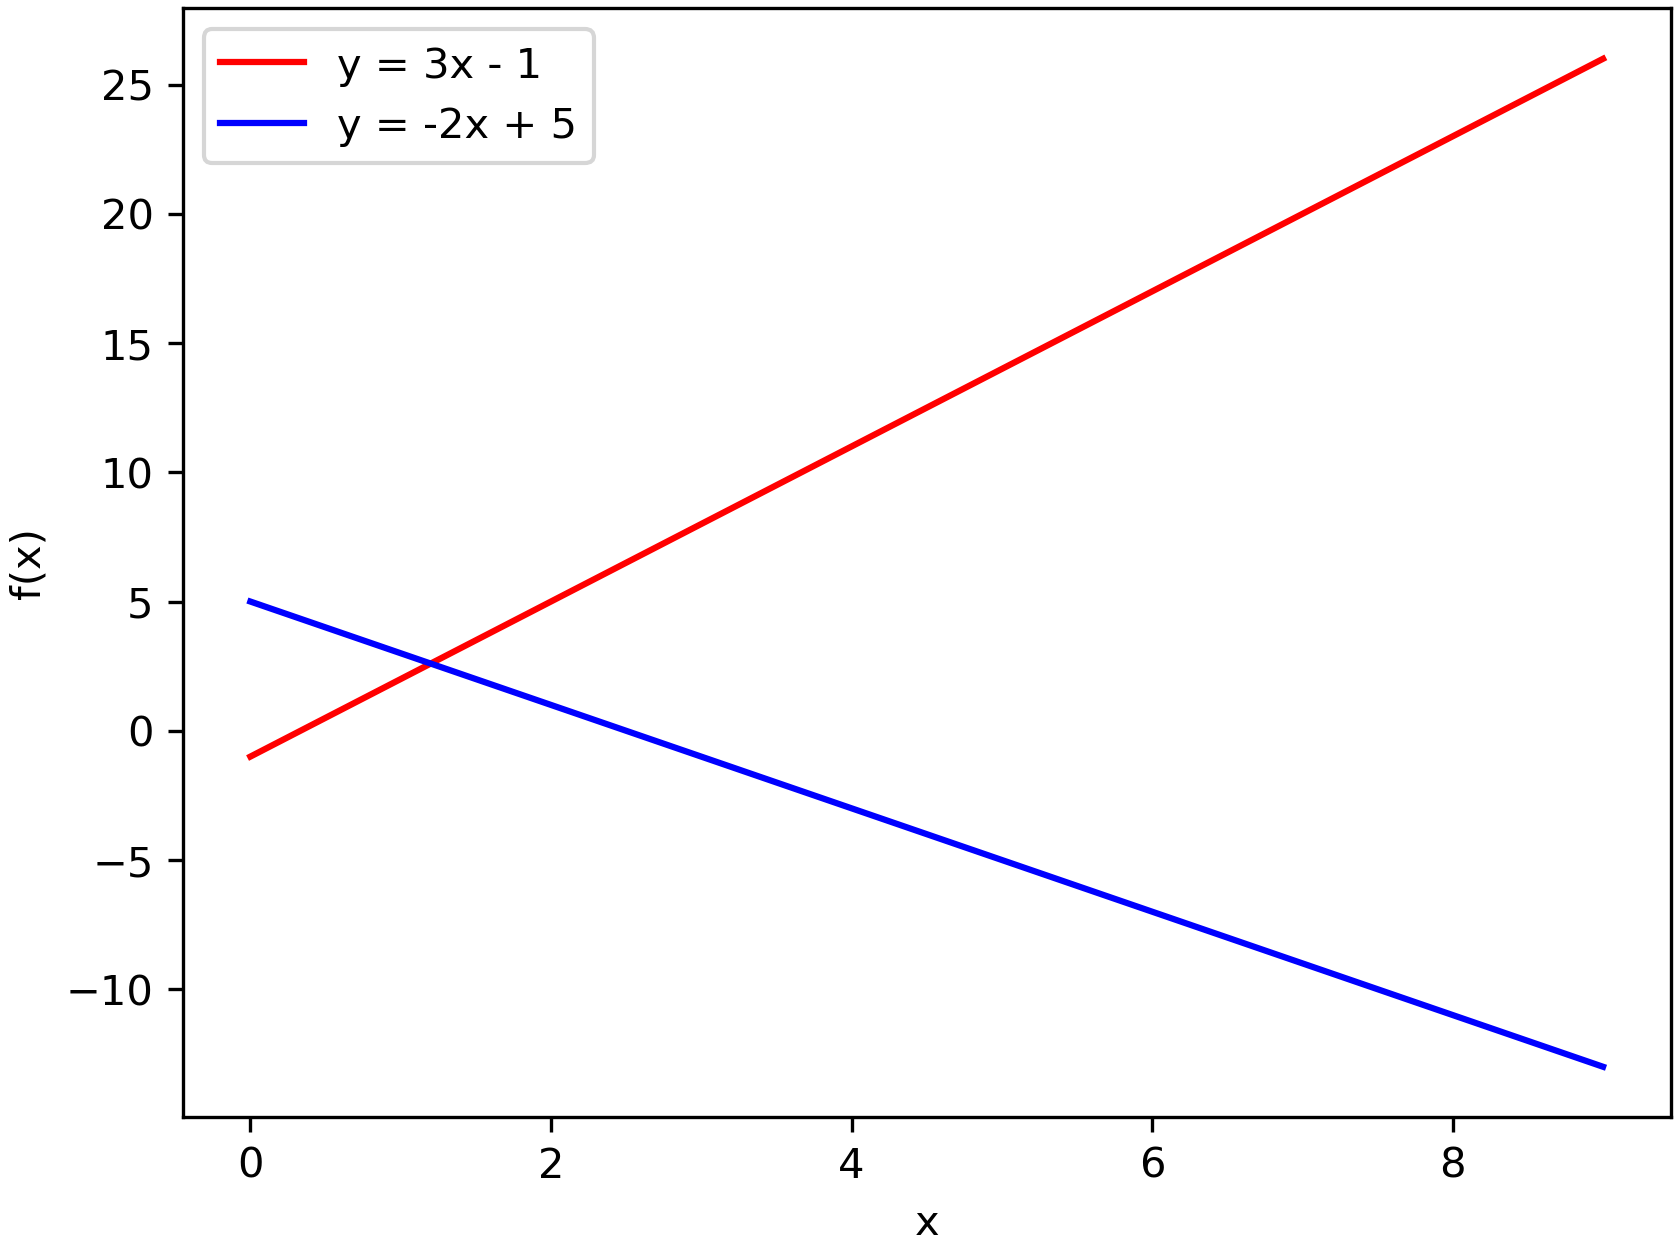
\includegraphics[width=0.7\textwidth]{figures/matplotlib_lines.png}

\subsubsection{Gráfico de histogramas}
Para crear un histograma se utiliza la función <<\pynorm{hist()}>>. Por ejemplo, podemos crear un arreglo aleatorio que sigue una distribución normal y visualizarlo con \pynorm{matplotlib}:

\begin{pyin}[]
#- Distribución normal
x = np.random.normal(100, 20, 100)

#- Dibujar el histograma
plt.hist(x)

#- Añadir etiquetas a los ejes
plt.xlabel('Valores')
plt.ylabel('Frecuencia')

#- Muestra la figura
plt.show()
\end{pyin}

\noindent
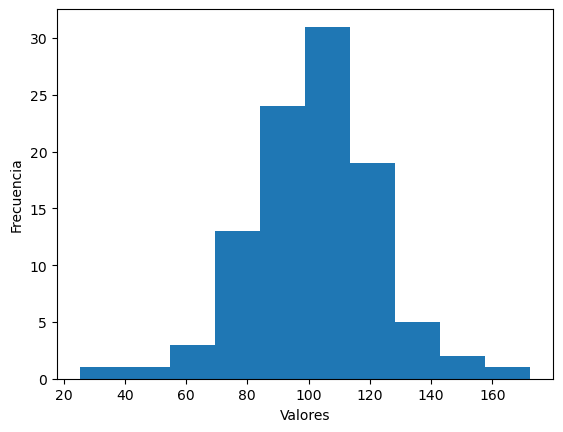
\includegraphics[width=0.7\textwidth]{figures/matplotlib_hist.png}

\subsubsection{Visualización de matrices}
Para visualizar matrices en Python, se utiliza la función <<\pynorm{imshow()}>> definida en \pynorm{matplotlib.pyplot}. Por ejemplo, vamos a usar una de las funciones de \pynorm{numpy.random} para generar una matriz con números aleatorios y luego visualizarlos.

\begin{pyin}[]
#- Matriz de 100x100 con números aleatorios
matrix = np.random.random((100, 100))

#- Dibuja la matriz
plt.imshow(matrix)

#- Muestra la barra de colores
plt.colorbar()
plt.show()
\end{pyin}

\noindent
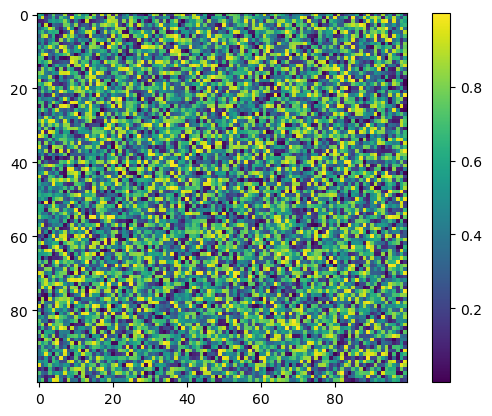
\includegraphics[width=0.7\textwidth]{figures/matplotlib_matrix.png}

\subsubsection{Gráfico de una función de dos variables}
Matplotlib también permite visualizar gráficas de contorno para funciones de la forma $ z = f(x, y) $. Por ejemplo, comencemos definiendo una función en Python que represente este tipo de funciones matemáticas:

\begin{pyin}
def f(x, y):
    return np.sin(x) ** 10 + np.cos(10 + y * x) * np.cos(x)  
\end{pyin}

Para crear un gráfico de contornos se utiliza la función <<\pynorm{plt.contour()}>> que toma tres argumentos: una malla de valores de $ x $, otra malla de valores de $ y $ y una malla de valores de $ z $. Para crear este tipo de arreglos necesitamos de la función <<\pynorm{np.meshgrid()}>>, que genera una malla bidimensional a partir de arreglos unidimensionales.

\begin{pyin}[]
#- Valores de x e y
x = np.linspace(0, 5, 50)
y = np.linspace(0, 5, 40)

#- Malla de x e y
X, Y = np.meshgrid(x, y)

#- Malla de valores de z
Z = f(X, Y)
\end{pyin}

Y ahora podemos visualizar la función:

\begin{pyin}
plt.contour(X, Y, Z, colors='black')
plt.show()
\end{pyin}

\noindent
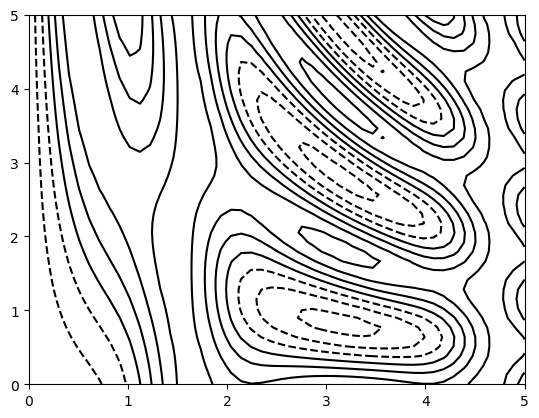
\includegraphics[width=0.7\textwidth]{figures/matplotlib_contour.png}

Como último ejemplo, veamos cómo graficar una función gaussiana en dos dimensiones, que tiene la forma:
\[
f(x, y) = \frac{1}{2\pi\sigma_x\sigma_y} \exp\left(-\frac{1}{2}\left[\left(\frac{x - \mu_x}{\sigma_x}\right)^2 + \left(\frac{y - \mu_y}{\sigma_y}\right)^2\right]\right).
\]

Comenzamos definiendo los valores de $ x $ y $ y $:
\begin{pyin}[]
#- Definir la cuadrícula de puntos
x = np.linspace(-3, 3, 100)
y = np.linspace(-3, 3, 100)
X, Y = np.meshgrid(x, y)
\end{pyin}

Y ahora podemos establecer los parámetros de la distribución gaussiana en dos dimensiones:
\begin{pyin}[]
#- Media
mu_x, mu_y = 0, 0  

#- Desviación estándar
sigma_x, sigma_y = 1, 1  
\end{pyin}

Y ahora calculamos los valores de la distribución:
\begin{pyin}
Z = (1 / (2 * np.pi * sigma_x * sigma_y)) * np.exp(-((X - mu_x)**2 / (2 * sigma_x**2) + (Y - mu_y)**2 / (2 * sigma_y**2)))
\end{pyin}

Finalmente, visualizamos. Esta vez utilizaremos la función <<\pynorm{plt.contourf()}>> que es igual a \pynorm{plt.contour}, pero rellena de color los contornos. Además, usaremos el mapa de colores llamado <<\pynorm{viridis}>>:

\begin{pyin}
plt.contourf(X, Y, Z, cmap='viridis')
plt.colorbar(label='Densidad de probabilidad')
plt.title('Distribución Gaussiana en 2D')
plt.xlabel('X')
plt.ylabel('Y')
plt.show()
\end{pyin}

\noindent
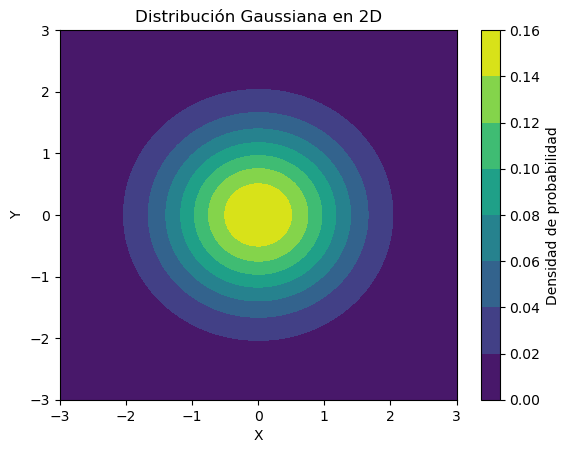
\includegraphics[width=0.7\textwidth]{figures/matplotlib_2d_gaussian.png}
